\documentclass[../main.tex]{subfiles}

\begin{document}

\section{Lecture 11}{Eigenvalue Problems}


\begin{definition}
    ALgebraic multiplicity of an eigenvalue counts the number of times the eigenvalue occurs as a root of the characteristic equation. Geometric multiplicity counts how many linearly independent eigenvectors correspond to an eigenvalue. It is a proveable fact that 
    algebraic multiplicity is at least as much as the geometric multiplicity. If algebraic multiplicity is greater than geometric multiplicity, we say that the matrix is defective.
\end{definition}

\begin{theorem}
    Similar matrices share the same eigenvalues.
\end{theorem}

\begin{theorem}
    If a matrix is defective, then it cannot have an eigenvector basis.
\end{theorem}

\begin{proposition}
    A matrix is diagonalizable iff it has an eigenvector basis.
\end{proposition}

\begin{proposition}
    The following matrix transformations change eigenvalues and eigenvectors as follows:

    \begin{outline}
        \1 $A \rightarrow (A - \sigma I)$ causes $\lambda \rightarrow \lambda - \sigma$. 
        \1 $A \rightarrow \inv{A}$ causes $\lambda \to \frac{1}{\lambda}$>
        \1 $A \rightarrow A^k$ causes $\lambda \to \lambda^k$.
        \1 If $A = PX\inv{P}$, then $X$ has the same eigenvalues but every eigenvector $v$ now becomes $\inv{P}v$.
    \end{outline}
\end{proposition}

\begin{proposition}
    Suppose that we perturb a diagonal matrix $A$ with some matrix $E$. Then the distance between any eigenvalue $u$ of $A + E$ to an eigenvalue of $A$ $\lambda_k$ closest to $u$ is bounded by $k(A) \norm{E}$.
\end{proposition}

\section{Lecture 12}

\begin{problem}
    Characteristic Polynomial
For which of the following reasons is the characteristic polynomial of a matrix NOT useful, in general, for computing the eigenvalues of the matrix?

Select all that apply:
Its coefficients may not be well determined numerically.
Its roots may be difficult to compute.
Its roots may be sensitive to perturbations in the coefficients.
None of these
\end{problem}

\begin{solution}
    Yes, the roots change if the coefficients change -- hence any perturbation will affect the roots; determining the coefficients numerically is also problematic, simply because numerical comptutation requires rounding error and truncation error. The second is a given.
\end{solution}

\begin{problem}
    Problem Transformations and Spectral Radius
Which of the following transformations preserve the spectral radius of a matrix A?

Select all that apply:
Powers
None of these
Shift
Polynomial
Inversion
\end{problem}
\begin{solution}
    Obviously, none of them, since they all change the eigenvalues.
\end{solution}

\begin{problem}
    Diagonalizability
Of the classes of n×n matrices listed below, which is the smallest class of matrices that are not necessarily diagonalizable by a similarity transformation?

Choice*
normal matrices
all matrices
real symmetric matrices
matrices with n distinct eigenvalues
\end{problem}
\begin{solution}
    A spectral theorem asserts that normal matrices are unitarily diagonalizable; a theorem asserts that real symmetric matrices have an orthogonal basis -- hence they are diagonalizable; in general, any matrix with an eigenbasis is diagonalizable.
\end{solution}

\begin{problem}
    Let $A = XD\inv{X}$. Suppose $\hat{A} = A + \delta A = \hat{X} \hat{D} \inv{(\hat{X})}$. Which matrix is $\hat{A}$ similar to?
\end{problem}

\begin{solution}
    $\inv{X}\hat{A} X = \inv{X}AX + \inv{X}\delta A X = D + \inv{X} \delta A X$
\end{solution}

\begin{definition}
    The eigenvector corresponding to the largest eigenvalue will hence forth be called the maximal eigenvector. 
\end{definition}

\begin{remark}
    Power iteration can fail because of certain reasons; certain of these can be remedied:

    \begin{outline}
        \1 No component alongside the dominant eigenvector.
        \2 Rounding error usually introduces some component -- and a random vector will usually include the component.
        \1 Overflow of entries in the vector being iterated upon:
        \2 Normalize the vector
        \1 There is no one dominant eigenvector, because two distinct eigenvalues of equal, maximal magnitude exist.
    \end{outline}
    
\end{remark}

\begin{definition}
    The rayleight quotient is the quantity

    \[
        \frac{x^T Ax}{x^Tx}
    \]
\end{definition}

\begin{remark}
    Let $e_k = \norm{v_1^{k} - x_1}$ where $v_1^k$ is the estimate of $x_1$ at the $k$th iteration.

    It can be shown that error $\approx c \abs{\frac{\lambda_2}{\lambda_1}}^k$, which implies that

    \[
        \frac{\norm{e_{k+1}}}{\norm{e_k}} = \abs{\frac{\lambda_2}{\lambda_1}}
    \]

    This is called linear convergence, because the error in the next iteration is a linear (think $y = ax$) scaling of the previous error.

    Power iteration obviously costs $O(n^2)$ at each iteration, because we're repeatedly multiplying a matrix by a vector.
\end{remark}

\begin{definition}
    Inverse power iteration is the algorithm that repeatedly hits $x$ with $\inv{A}$. Its statistics:

    \begin{outline}
        \1 The error rate is 

        \[
            \frac{\abs{1/\lambda_{n-1}}}{\abs{1/\lambda_{n}}} = \frac{\abs{\lambda_n}}{\abs{\lambda_{n-1}}} 
        \]
        \1 The cost is initially $O(n^3)$ since we solve for $y$ in $Ay = x$. Thereafter, the cost is $O(n^2)$.
        \1 The largest eigenvalue is $\abs{\frac{1}{\lambda_n}}$
    \end{outline}
\end{definition}

\begin{definition}
    Shifted inverse power iteration iterates on $x$ using $\inv{(A - \sigma I)}$. \\

    The dominant eigenvector corresponds to the eigenvalue $\frac{1}{\lambda' - \sigma}$ where $\lambda'$ is the closest eigenvalue of $A$ to $\sigma$. If $\lambda''$ is the second closest eigenvalue to $A$ then the error rate is given by 

    \[
        \frac{\abs{\lambda' - \sigma}}{\abs{\lambda'' - \sigma}}
    \]

    The cost is initially $O(n^3)$ but then $O(n^2)$ thereafter.

\end{definition}

\begin{definition}
    Shifted Rayleigh iteration leverages both power iteration and the Rayleight quotient method in order to determine the maximal eigenvector:
    \begin{outline}
        \1 Compute the rayleigh quotient to obtain $\sigma_k$.
        \2 Multiply $\inv{(A -\sigma_k I)}$ by $x_k$.
        \3 In reality, by multiplication, we mean compute the
        LU factorizaton of $A - \sigma_k I$ and then use it
        \1 This will presumably give us an eigenvector that corresponds
        to the eigenvector closest to $\sigma$.
        \2 Note that $\sigma$ was not chosen with any prior intent however -- it just happens to be our estimate of the eigenvalue that corresponds to some initial $x$, and that initial $x$ is our estimate of some eigenvector.
        to compute the multiplication.
        \1 This is good, because it can be shown to converge
        at a quadratic rate -- whereas ordinary power iteration
        convergence is linear.
        \2 This is bad, because we have to factor
        $A - \sigma_k I$ every iteration, which can be expensive.
        \2 This may not also converge to an eigenvector we want to converge to apriori.
    \end{outline}
\end{definition}


\begin{definition}
    Simultaneous iteration seeks to determine the maximal $p$ eigenvectors; or rather a basis for them.
    \begin{algo}
        Initialize some $X_0$, an $n \times p$ matrix. \\
        $X_{k+1} = AX_{k}$ \\
        \redcomment{You can perform orthonormalization if needbe} \\
    \end{algo}
\end{definition}

\begin{remark}
    This algorithm is problematic, because the column vectors in $X_k$ may tend to the dominant eigenvector. As a result, $X_k$ becomes increasingly more and more ill conditioned. This is bad, in and of itself, because we typically desire that $X_k \to X$, which we define to be a basis for the span of the dominant $p$ eigenvectors.
\end{remark}

\begin{definition}
    One remedy to this problem is to orthonormalize the iterate of the basis:

    In what follows, assume that we use the full unreduced $QR$ factorization.

    \begin{algo}
        Initialize some $Q_0$, corresponding to our guess \\
        of a basis for the dominant $p$ eigenvectors.\\
        $Q_0$ is an orthogonal matrix that is $n \times n-p$ \\
        While $\norm{Q_{k+1} - Q_{k}} > \text{some tolerance}$ \+\\
        $X_{k+1} \coloneq AQ_{k}$ \\
        $Q_{k+1}R_{k+1} \coloneq X_{k+1}$ \\
    \end{algo}

    Notice that at each iteration, we have $A = Q_{k+1}R_{k+1}Q_{k}^T$. If $Q_k \to Q$ then $A = QRQ^{T}$ ($R$ also converges as a consequence), so that we have found some (allegedy dominant) $p$ eigenvectors in $Q$ and their eigenvalues in the $p \times p$ upper triangular $R$.
\end{definition}

\begin{remark}
    Assume now that we use the reduced $QR$ factorization so that $Q$ is $n \times r$ and $R$ is $r \times r$.

    The span of $Q_k$ is the span of $X_k$ at any point. Thus $X_{k+1} = A Q_{k}$ gives us a set of column vectors whose span is the same as the span of $AX_{k}$. Thus, we can use $Q_k$ as a proxy to $X_k$.

    Why is span$(Q_k) = $span$(X_k)$ -- since otherwise, the $QR$ factorization of $X_k$ (which we assume to be of rank $r$ -- or else -- we are not determining distinct eigenvectors) will reduce the rank of $X_k$.
\end{remark}



\begin{definition}
    In $QR$ iteration, we decompose $A_k$ as $Q_kR_k$ and then obtain $A_{k+1} = R_kQ_k$. Notice that $A_{k+1} = Q_{k}^TA_kQ_k$ so that if $Q_k$ converges then $A_{k+1}$ is now (this is not yet underestood) really an upper triangular matrix with eigenvalues along its diagonal.
\end{definition}

\begin{definition}
    In $QR$ iteration with shifting, we factor $A_k - \sigma_k I$ as $Q_k R_k$ and then compute

    \[
        A_{k+1} = R_k Q_k + \sigma I
    \]

    Note that since $R_k = Q_k^T(A_k - \sigma_k I)$, it follows that

    \[
        A_{k+1} = Q_k^T(A_k - \sigma_k I)Q_k + \sigma I = Q_k^T A_k Q_k
    \]
\end{definition}

\begin{definition}
    The Schur decomposition of a matrix $A = QUQ^H$ expresses $A$ as similar to an upper triangular matrix $U$. A proof of this theorem is given in \url{http://people.inf.ethz.ch/arbenz/ewp/Lnotes/chapter2.pdf} at page 6. We now list some properties pertaining to the matrix:

    \begin{outline}
        \1 Since $AQ = QU$, we can conclude that $AQ_1 = Q_1(U_{1,1})$. From this, it follows that the first schur vector $Q_1$ is an eigenvector.
        \1 If $Q$ and $U$ are real, then $QU$ is a $QR$ decomposition -- obviously.
        \1 If $A$ is real symmetric, then it must be true that $U$ is diagonal, in which case it contains all the eigenvalues of $A$. 
        \2 Moreover, since $U = Q^HAQ$, one can shown that $U^{*} = U$, implying that all the eigenvalues are real. A proof near the proof listed above additionally explains that eigenvectors corresponding to distinct eigenvalues are orthonormal.
    \end{outline}<++>
\end{definition}<++>

\section{Lecture 13}

\begin{problem}
    Suppose we are given the matrix

    \[
        A = \begin{bmatrix}
            1 & 0 \\
            3 & 0.1 \\
        \end{bmatrix}
    \]

    Then how many power iterations do we need in order to reduce the error by $10^{-10}$.
\end{problem}
\begin{solution}
    The convergence rate is given by $\abs{\frac{\lambda_2}{\lambda_1}}$; hence the rate is $10^{-1}$ and we need at least $10$ iterations. Note that we additionally assume that the starting vector has components in both directions corresponding to the eigenvalue.
\end{solution}

\begin{problem}
    Assume that we are given an $LU$ factorization from a previous computation. What is the cost of performing inverse power iteration for $k$ iterations on an $n \times n$ matrix.
\end{problem}

\begin{solution}
    The cost is $O(kn^2)$. Recall that $LU$ factorizations, once calculated, allow us to solve inverse problems in $O(n^2)$ time.
\end{solution}

\begin{problem}
    Estimate the rayleight quotient of a given matrix for a given eigenvector. Trivial; whence the solution is ommitted.
\end{problem}

\begin{problem}
    Properties of the Schur Form
 Consider the Schur decomposition of a matrix A=QUQH where U is upper-triangular and Q is unitary. The Schur vectors are the columns of Q. While of the following are true?

Select all that apply:
If A is real, Q is orthogonal and U is real
The first Schur vector is an eigenvector of A
The Schur form of a matrix is unique so long as its eigenvalues are not all the same
If A is real symmetric, the Schur decomposition is the eigenvalue decomposition of A
If Q and U are real, QU is a QR decomposition of AQ
    
\end{problem}
\begin{solution}
    \begin{outline}
\1 If A is real, Q is orthogonal and U is real
\2 $A$ coudl be real but $Q$ and $U$ still complex.
\1 The first Schur vector is an eigenvector of A
\2 True -- see above.
\1 The Schur form of a matrix is unique so long as its eigenvalues are not all the same
\2 In the proof of the schur decomposition, the eigenvalue (which is entry occupying the first diagonal entry of $\Lambda$)  was chosen without any specificity -- so that any eigenvalue can be chosen there.
\1 If A is real symmetric, the Schur decomposition is the eigenvalue decomposition of A
\2 Yes, see above.
\2 If Q and U are real, QU is a QR decomposition of AQ.
\2 Yes, can be observed from the form of the schur decomposition itself.
    \end{outline}
    
\end{solution}

\begin{problem}
    QR Iteration for Special Matrices
Which of the following statements about doing one iteration of QR decomposition on a matrix A∈ℝn×n is true?

Select all that apply:
For a Hessenberg matrix A, it takes O(n2) time.
For a Hessenberg matrix A, it takes O(n3) time.
For a tridiagonal matrix A, it takes O(n) time.
For a tridiagonal matrix A, it takes O(n2) time.
\end{problem}

\begin{solution}
    Imagine that we use Givens' rotations. Take the $k$th column as an example. After finding the rotation that takes the $k+1$th row to the $k$th row, we need to apply this same rotation to the remaining $n-k$ columns to the right of the $k$th column. Thus, even if the givens' rotation takes $O(n)$ time to both compute and apply its effects to the $k$the column, the cost of its application to the remaining columns results in $O(n^2)$. By contrast, in a tridiagonal matrix, after finding the rotation that ``settles'' the $k$th column, the rotation only need be applied to the $k+1$th column, since the rotation will change the $k$th entry of that column; no other column to the right will be affected. Thus, this results in an $O(n)$ cost.
\end{solution}

\begin{remark}
    To arrive at the schur form of a matrix, we need to perform some unspecified number of $QR$ factorizations. Each factorization takes $O(n^3)$. Thus the cost can often near $O(n^4)$.
\end{remark}

\begin{remark}
    A better technique is to use a trick involving Householder Transformations:

    \begin{outline}
        \1 Having computed a householder vector $h_i$ that nullifies everything beneath and including row $i+2$, and having formed $H_i$ which is the transformation that achieves this, carry out $H_i A (H_i)^T$. What will this do? It can be shown that this will zero out all entries past and including the $i+2$ row. Doing this for each column, we will attain Hessenberg form. Having attained Hessenberg form. That is $A = \prod_{i=1}^{n}(H_i)^T H (\prod_{i=1}^{n}H_i)$,which is a similarity transform to $A$, meaning that the eigenvalues for $A$ are contained in $H$. We can now perform $QR$ iteration on $H$. It costs $O(n^2)$ to perform the necessary number of Givens rotations to $QR$ factorize the matrix. Suppose that we obtain at the very first iteration the factors $Q_1R_1 = H$. Observe that $A_{2} = R_1Q_1 = R_1H\inv{R_1}$. Further reacall that post or pre multiplying a Hessenberg matrix by an upper triangular matrix preserves the form of the Hesenberg matrix. It therefore follows that $A_2$ is Hessenberg as well; thus every $QR$ iteration now requires $O(n^2)$ as opposed to $O(n^3)$.
    \end{outline}
\end{remark}

\begin{remark}
    In a Krylov subspace method, we restrict our focus to finding a few eigenvect   
\end{remark}<++>

\begin{definition}
    \begin{outline}
        \1 Suppose that we begin with an initial vector $x_0$. Let

        \[
            K_n = \begin{bmatrix}
                x_0 & Ax_0 & \dots & A^{n-1}x_0   \\
            \end{bmatrix}
        \]

        Observe  that 

        \begin{align*}
            AK_n  = \begin{bmatrix}
                   Ax_0 & A^2x_0 & \dots & A^{n}x_0   \\
            \end{bmatrix}
            = K_n
            \underbrace{\begin{bmatrix}
                e_2 & e_3 & \dots & e_n &  \inv{K_n}A^nx_0
            \end{bmatrix}}_{H} 
        \end{align*}

        That is we found that $\inv{K_n}AK_n = H$, where $H$ is upper Hesenberg.
    \end{outline}
\end{definition}

\begin{remark}
    So what? Why is this important? We wish to work with $H$ to determine its eigenvalues.
    The foregoing reveals that we will need to compute $K_n$ if we wish to compute $H$. The problem is that $K_n$ will tend to multiples of the dominant eigenvector of $A$, since $K_n$ is obtained by performing power iteration a few times on $x_0$. This makes $K_n$ highly ill conditioned, so that the Hesenberg form that we would obtain by mat-mat multiplication is likely not useful. What we will therefore do is that we will find a $Q_nR_n$ factorization for $K_n$.
\end{remark}

\begin{remark}
    \begin{align*}
        Q_n^HAQ_n = \inv{(K_nR_n)} A (K_nR_n) = \inv{(R_n)}\inv{K_n}K_nK_n R_n = \inv{(R_n)}HR_n \cong C
    \end{align*}
    17

    where $C$ is some Hesenberg matrix in addition to $H$.
\end{remark}

\begin{proposition}
    The vectors of $Q_n$ can each be computed alone.
\end{proposition}
\begin{proof}
    \begin{align*}
        AQ_n = Q_nC \\
        \intertext{For notational convenience, let $Q =Q_n$} \\
        \intertext{Let us focus on the $j$th column. Suppose that $Q_n$ = }
            \begin{bmatrix}
                q_1 & q_2 \dots q_n
            \end{bmatrix}
            \implies Aq_j = \sum_{i=1}^{j+1}q_{i}C_{i,j} \\
            \intertext{Now solve for $q_2$ assuming that we know $q_1$ and that we have orthonormalized $q_1$. This gives us:}
            \implies Aq_1 = \sum_{i=1}^{2}q_{i}C_{i,1} \\
            \implies Aq_1 = q_{1}C_{1,1} + q_{2}C_{2,1} \\
            \implies Aq_1 - q_{1}C_{1,1} = q_{2}C_{2,1} \\
            \intertext{Note that $Aq_1$ is the ``next'' vector in a Krylov subspace that one would compute with knowledge of $q_0$.} \\
    \end{align*}

    Now in general $C_{i,j} = q_i^HAq_j$. In particular $C_{1,1} = q_1^HAq_1$. If we let $u_1 = (Aq_1)$, then we see that $C_{1,1} = q_1^H u_1$ and that 

    \[
        Aq_1 - q_{1}C_{1,1} = u_1 - q_{1} C_{1,1}
    \]

    This is tantamount to orthogonalizign $u_1$ by removing all of the projections of $u_1$ onto previous $q_k$ (in this case, only $q_1$). Thus if we set $q_2 = \frac{u_1}{\norm{u_1}}$, then we will have effectivel found the vector $q_2$ that is part of the orthonormal set of Krylov space vectors.
\end{proof}

\begin{remark}
    This can be formalized as part of an algorithm:

    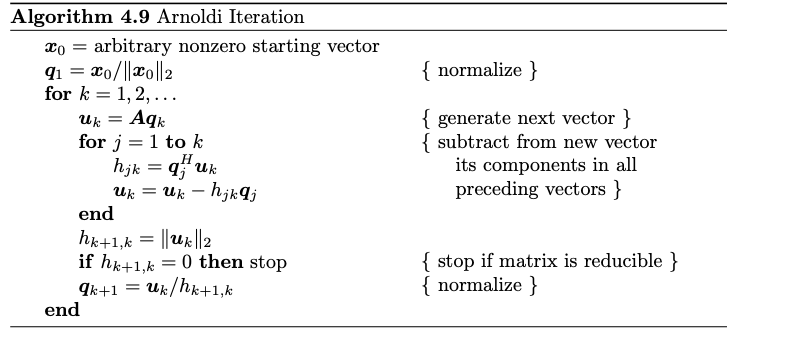
\includegraphics[width=\textwidth,height=\textheight,keepaspectratio]{lecture13_arnoldi}
\end{remark}

\begin{proposition}
    We can compute the eigenvectors corresponding to the $k$ greatest eigenvalues in modulus.
\end{proposition}

\begin{proof}
    We found that $Q_n^h A Q_n \cong H$, an upper Hesenberg matrix. Define 
    \[
        Q_{k} = \begin{bmatrix}
            q_1 & \dots q_k
        \end{bmatrix}
    \]

    to be the $n \times k$ matrix that consists of the first $k$ Arnoldi vectors. Define

    \[
        U_{k} = \begin{bmatrix}
            q_{k+1} & \dots q_{n}
        \end{bmatrix}
    \]

    to be the matrix consisting of the remaining $k$ uncomputed vectors. It follows that

    \begin{align*}
        Q_n^H A Q_n = 
        \begin{bmatrix}
            Q_k^h \\
            U_k^h
        \end{bmatrix}
        A
        \begin{bmatrix}
            Q_k & U_k
        \end{bmatrix}
    \end{align*}
\end{proof}

\section{Lecture 14}{Nonlinear equations}
\begin{problem}
    QR Iteration Convergence
For which of the following classes of matrices will QR iteration always converge and produce all the eigenvalues?

Select all that apply:
Symmetric matrix
Diagonal matrix
Orthogonal matrix
Upper Triangular matrix
General matrix with complex eigenvalues
\end{problem}

\begin{solution}
    Stupid trick question. The answer is a diagonal matrix and an upper triangular matrix. For we don't need to invoke the $QR$ algorithm on these matrices; we already know their eigenvalues (just read the diagonal).
    
    $QR$ is never guaranteed to always converge (ie in a finite number of steps), because there is proveably no algorithm that can give us the eigenvalues for matrices with length at least $5$. 
\end{solution}

\begin{problem}
    Krylov Subspace Conditioning
Given a matrix A with condition number κ=100 and an initial vector x0, how many additional Krylov vectors can be calculated while ensuring the relative error of each vector remains less than or equal to 1×10−6 assuming IEEE double precision.
\end{problem}
\begin{solution}
    The answer is $5$. The relative error is bounded by the condition number multiplied by the relative input error. At the $k$th iteration the relative input error is the relative output error of the $k-1$th iteration where the relative input input error of the $0$th iteration is given by machine epsilon, ie $\approx 2 \times 10^{-16}$. Therefore, relative output error at iteration $k$ is $100^k 2 \times 10^{-16}$, meaning that we can let $k$ be at most $5$.
\end{solution}

\begin{problem}
     Suppose A is a general n×n matrix and Q=[q1q2…qk] is an orthogonal matrix with qj∈Kj(A,b), the Krylov subspace associated with A. How many nonzero elements are in the matrix QTAQ?
\end{problem}
\begin{solution}
    See the notes previously that explain that if we gather the fist $k$ Arnoldi vectors into a matrix $Q$ then $Q^T A Q$ is upper Hesenberg and $k \times k$, meaning it has $k^2$ non zero entries. 
\end{solution}

\begin{problem}
    Qk is the matrix obtained by orthogonalizing the columns of

Ck=[bAbA2b…Ak−1b].
Which of the following is equal to QTkb?
\end{problem}

\begin{solution}
    $Q_k$ will contain column vectors such that only the first vector $q_1$ is orthonormal with $b$. In fact that $\inner{q_1, b} = \inner{q_1, \frac{b}{\norm{b}}\norm{b}} = \norm{b}\inner{q_1, \frac{b}{\norm{b}}} = \norm{b} e_1$.
\end{solution}

\begin{problem}
    Coding question:
\end{problem}

\begin{solution}
    Here the solution is to recall that once we factorize $K_n = Q_nR_n$ then the upper Hesenberg matrix $K_n^T A K_n$ can be alternatively be expressed as

    \[
        Q_n^T A Q
    \]

    since this simplifies to

    \[
        R_n \inv{K_n} A K R_n
    \]

    which is still upper Hesenberg.
\end{solution}<++>











\end{document}
